\documentclass[11pt]{extarticle}

\usepackage[margin=1in]{geometry}
\usepackage[english]{babel}

\usepackage{amsmath}
\usepackage{graphicx}
\graphicspath{ {./figures/} }
\usepackage{caption}
\usepackage{subcaption}

\title{TXGL Midsemester Report}

\begin{document}
    \maketitle

    Our original goal which we set out to accomplish was to create a projection model of a flat, equilateral triangle with a shadow projected from a light source at a fixed point. The orientation of the triangle could be rotated while maintaining a fixed position; depending on how the triangle was rotated and where the light source is positioned, the size and shape of the shadow changed. Initially we were studying just the shape of a rotating triangle’s shadow in space. Due to the symmetry of an equilateral triangle, we determined that this particular kind of triangle could be rotated in such ways that any other shape of triangle could be created from its projected shadow. The rotation of the triangle was based on 9 total parameters on the x-y-z three-dimensional planes.

    \begin{figure}[!ht]
        \begin{subfigure}{.5\textwidth}
            \centering
            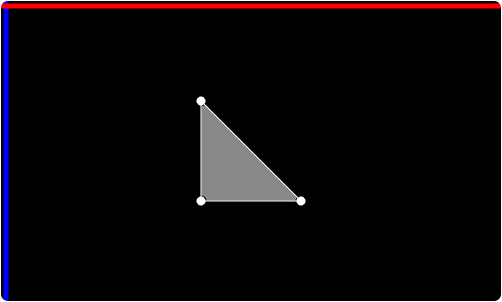
\includegraphics[scale=.5]{p5_1.png}
            \caption{Original triangle}
        \end{subfigure}
        \begin{subfigure}{.5\textwidth}
            \centering
            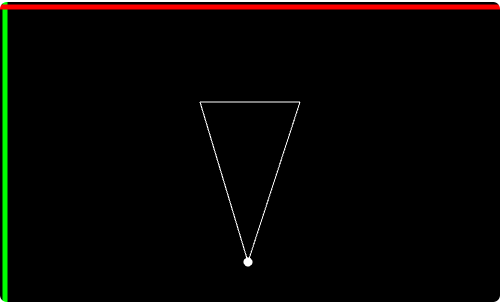
\includegraphics[scale=.5]{p5_2.png}
            \caption{Light source's XY coordinates}
        \end{subfigure}
        \\
        \begin{subfigure}{.5\textwidth}
            \centering
            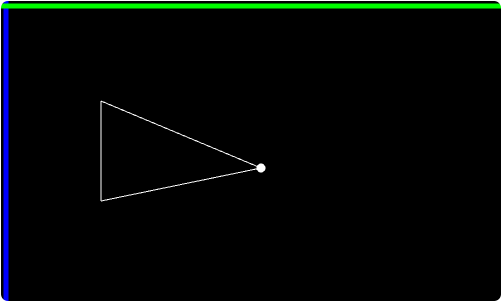
\includegraphics[scale=.5]{p5_3.png}
            \caption{Light source's YZ coordinates}
        \end{subfigure}
        \begin{subfigure}{.5\textwidth}
            \centering
            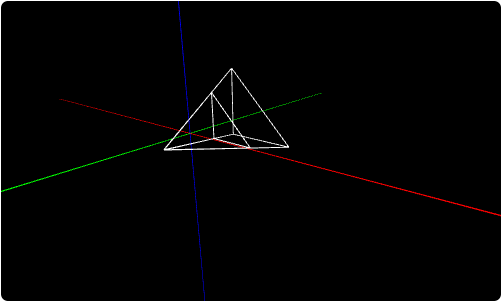
\includegraphics[scale=.5]{p5_4.png}
            \caption{A 3D perspective of the projection}
        \end{subfigure}
    \end{figure}

	After this initial overview of triangle projection, we took our study to the next step by adding another variable of a “bug” on the triangle (a fixed point around the middle of the triangle which was projected as a singular point along with the shadow from the light source). By now using a translucent triangle, we studied how to reposition the triangle such that the bug’s shadow moves but the triangle’s shadow shape is maintained. Using Mathematica, we created models allowing us to rotate the triangle on its axis orthogonally and parallel to its face (spinning it, flipping it, etc.).

    \begin{figure}[!ht]
        \centering
        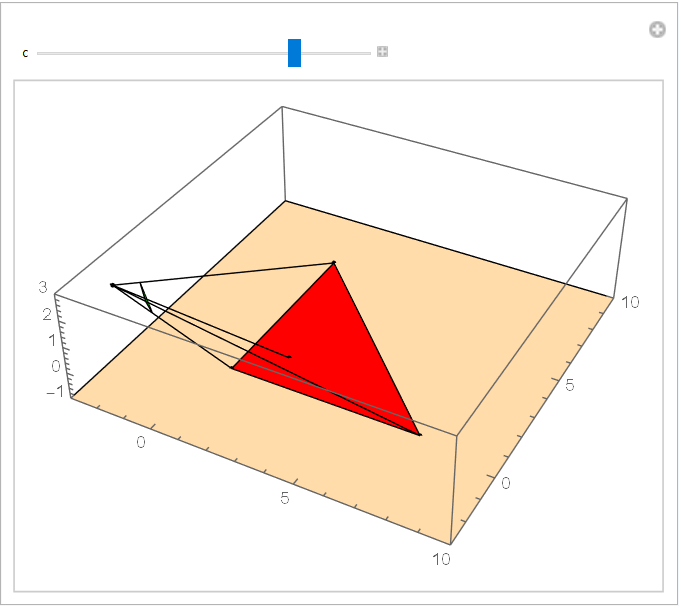
\includegraphics[scale=.5]{ma_triangle.png}
        \caption{Deriving the triangle from a fixed shadow with a fixed point projection in the middle. $C$ moves the light source along the $z$-axis. Projective plane ($z = 0$).}
    \end{figure}

	Our third and most recent discussion covers how to determine the roundness of a particular shape or object. With light projecting on a convex polygon, our goal is to find a way to maximize the roundness of the resulting shadow. In our research, we’re using a working definition of roundness, describing it as a minimization of the ratio between the radius of the circumscribed and inscribed circles of a polygon. In Mathematica, we were able to use functions including InCircle and InSphere to create a circle encompassing the whole of a particular shape while minimizing the radius of the circle (i.e., the smallest possible circle that could fit the entire shape). For example, we were able to find the in-circle of France as well as Japan.

    \begin{figure}[!ht]
        \begin{subfigure}{.5\textwidth}
            \centering
            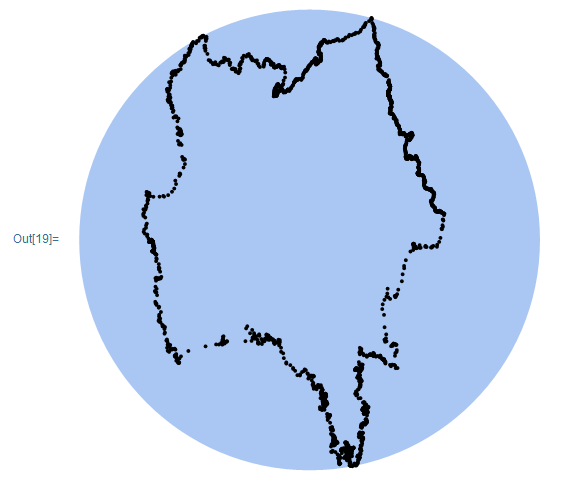
\includegraphics[scale=.35]{france.png}
        \end{subfigure}
        \begin{subfigure}{.5\textwidth}
            \centering
            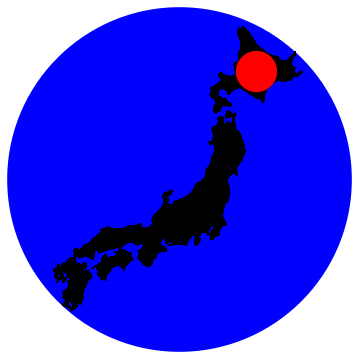
\includegraphics[scale=.5]{japan.png}
        \end{subfigure}
        \caption{The minimized-radius circles encompassing the shape of France and Japan, respectively}
    \end{figure}
\section*{Linear Projective Transformations}
The transformation matrix of a linear projective transformation is defined as
\[
\left( 
\begin{array}{ccc}
a & b & c \\
e & f & g \\
h & i & j \\
\end{array}
\right)
\]
which results in the transformation
\[
(X,Y) = \left( \frac{c + a x + b y}{j + h x + i y}, \frac{g + e x + f y}{j + h x + i y} \right) 
\]
where $(x,y)$ are the points on the projection before the transformation and $(X,Y)$ are points of the projection after the transformation.
    \begin{figure}[!ht]
        \centering
        \begin{subfigure}{.3\textwidth}
            \centering
            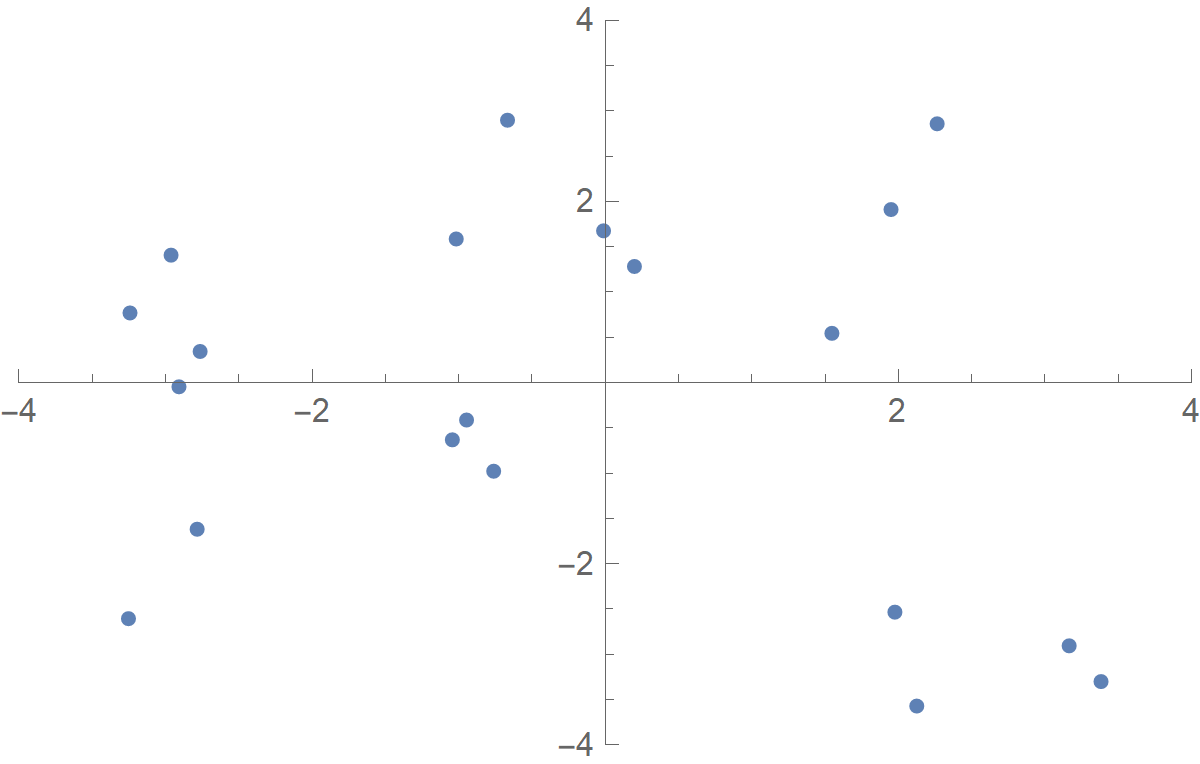
\includegraphics[scale=.1]{ma1.png}
            \caption{Original Projection}
        \end{subfigure}
        \begin{subfigure}{.3\textwidth}
            \centering
            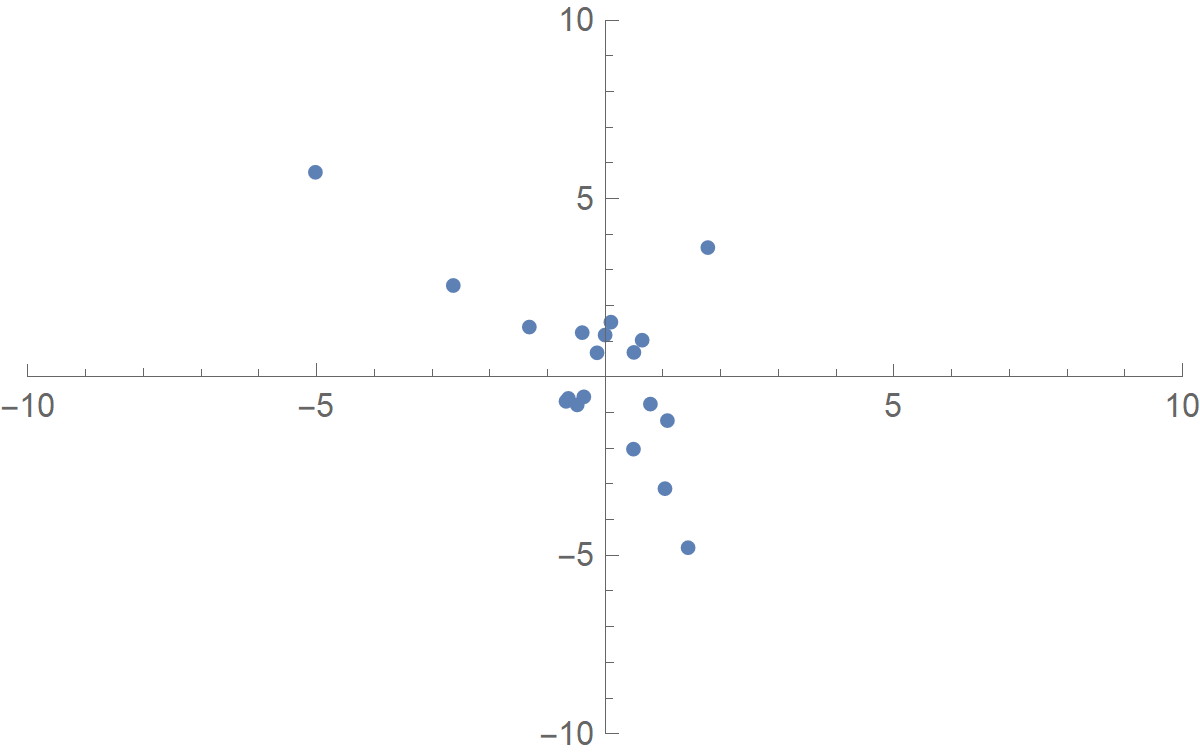
\includegraphics[scale=.1]{ma2.png}
            \caption{Transformed Projection}
        \end{subfigure}
        \begin{subfigure}{.3\textwidth}
            \centering
            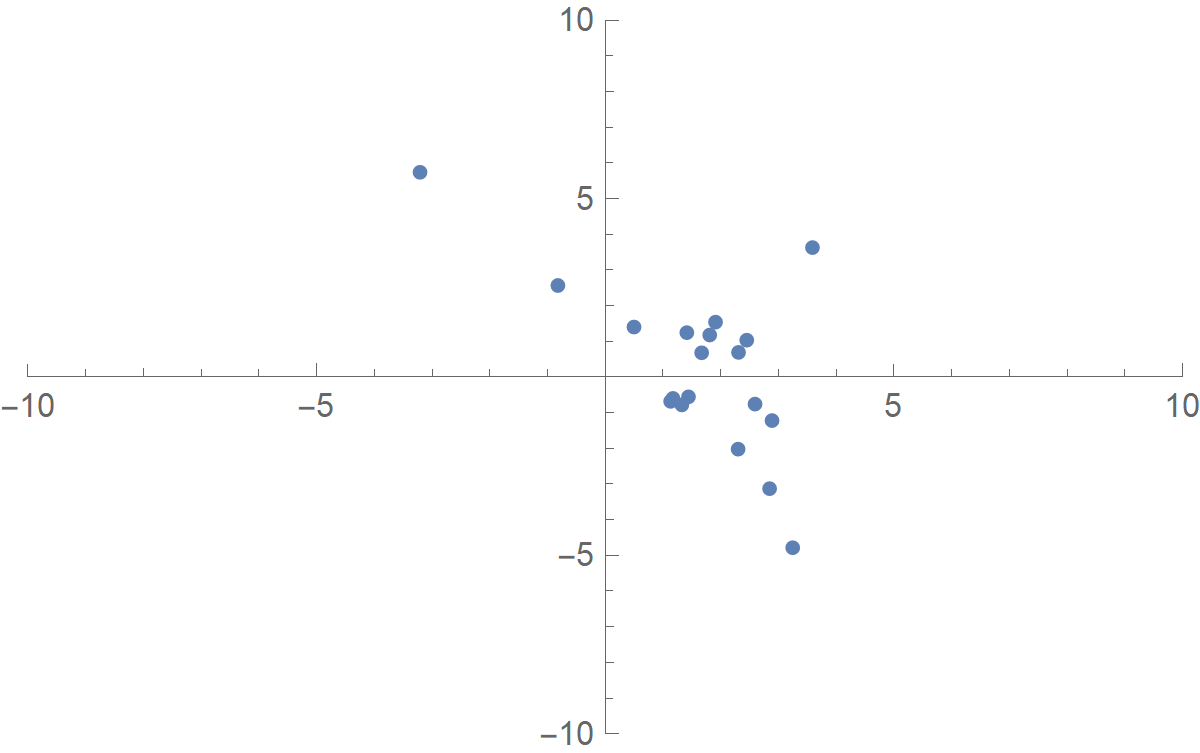
\includegraphics[scale=.1]{ma3.png}
            \caption{Different Transformation}
        \end{subfigure}
        \caption{(a) The original set of projected points. (b) An arbitrary linear projective transformation of those projected points. (c) When $h$ and $j$ of the transformation matrix are set to zero, changes in $b$ will shift the projection along the $x$-axis}
    \end{figure}
\end{document}